% !TeX program = xelatex
% Overleaf 编译器请选择 XeLaTeX。
\documentclass[UTF8,zihao=5,fontset=fandol]{ctexart}

\usepackage[a4paper,left=18mm,right=18mm,top=18mm,bottom=17mm,headheight=15pt,headsep=6mm]{geometry}
\usepackage{amsmath,amssymb,array,booktabs,enumitem,fancyhdr,lastpage,tabularx,tikz}
\usetikzlibrary{arrows.meta,automata,positioning}

\setlength{\parindent}{0pt}
\setlength{\parskip}{0pt}
\setlength{\abovedisplayskip}{4pt}
\setlength{\belowdisplayskip}{4pt}
\linespread{1.03}
\setlist[enumerate]{itemsep=4pt,topsep=4pt,parsep=0pt,partopsep=0pt,leftmargin=2em}

\pagestyle{fancy}
\fancyhf{}
\fancyhead[L]{\small 应用随机过程期中考试}
\fancyhead[R]{\small 第 \thepage\ 页，共 \pageref{LastPage} 页}
\renewcommand{\headrulewidth}{0.4pt}
\renewcommand{\footrulewidth}{0pt}

\newcommand{\blank}[1][3cm]{\underline{\hspace{#1}}}
\newcommand{\judgebox}{\hfill（\hspace{1.5em}）}
\newcommand{\sectiontitle}[1]{\vspace{3pt}{\zihao{4}\bfseries #1}\par\vspace{4pt}}
\newcommand{\fourchoices}[4]{%
  \begin{tabularx}{\linewidth}{@{}X X X X@{}}
    A.\,#1 & B.\,#2 & C.\,#3 & D.\,#4
  \end{tabularx}}
\newcommand{\twochoices}[2]{%
  \begin{tabularx}{\linewidth}{@{}X X@{}}
    A.\,#1 & B.\,#2
  \end{tabularx}}
\newcommand{\workarea}[1]{\vspace{#1}}

\begin{document}

%============================== 第 1 页 ==============================
\begin{center}
  {\zihao{3}\bfseries 杭州师范大学数学学院 2026--2027 第\blank[1.5em]学期期中考试}\par
  \vspace{4pt}
  {\zihao{4}\bfseries 考试科目：《应用随机过程》}\par
  \vspace{2pt}
  考试时间：120 分钟\hspace{4em}满分：100 分
\end{center}

\vspace{4pt}
\begin{tabularx}{\linewidth}{@{}l X l X l X@{}}
  姓名：&\hrulefill&学号：&\hrulefill&班级：&\hrulefill
\end{tabularx}

\vspace{6pt}
\begin{center}
\renewcommand{\arraystretch}{1.4}
\begin{tabular}{|c|c|c|c|c|c|}
  \hline
  题型 & 判断题 & 选择题 & 填空题 & 计算与应用题 & 总分 \\
  \hline
  得分 & \hspace{1.5cm} & \hspace{1.5cm} & \hspace{1.5cm} & \hspace{2cm} & \hspace{1.5cm} \\
  \hline
\end{tabular}
\end{center}

\sectiontitle{一、判断题（每题 1 分，共 10 分）}
请判断下列说法是否正确，正确写“$\checkmark$”，错误写“$\times$”。

\begin{enumerate}
  \item 若随机变量 $X$ 可积，则 $\mathbb{E}[\mathbb{E}(X\mid Y)]=\mathbb{E}X$。\judgebox
  \item 若随机过程 $\{X(t)\}$ 具有独立增量，则它一定具有平稳增量。\judgebox
  \item 对任意二阶随机过程，其协方差函数满足 $R_X(s,t)=R_X(t,s)$。\judgebox
  \item 若 $\{X(t)\}$ 为宽平稳过程，则 $\mathbb{E}X(t)$ 与 $t$ 无关，且 $\operatorname{Cov}(X(s),X(t))$ 只依赖 $t-s$。\judgebox
  \item 若 $\{N(t)\}$ 为强度 $\lambda$ 的 Poisson 过程，则
        $N(t)-N(s)\sim\operatorname{Poisson}(\lambda(t-s))$，$0\le s<t$。\judgebox
  \item 对 Poisson 过程，$N(s)$ 与 $N(t)$ 在 $0<s<t$ 时相互独立。\judgebox
  \item Poisson 过程的相邻到达时间间隔相互独立且服从同参数指数分布。\judgebox
  \item 在条件 $N(t)=n$ 下，$n$ 个到达时刻与 $n$ 个独立 $U(0,t)$ 随机变量的次序统计量同分布。\judgebox
  \item 有限不可约 Markov 链的每个状态都是正常返状态。\judgebox
  \item 只要有限 Markov 链存在唯一平稳分布，就一定有 $p_{ij}^{(n)}\to\pi_j$。\judgebox
\end{enumerate}

\sectiontitle{二、单项选择题（每题 2 分，共 20 分）}
\begin{enumerate}
  \item 设 $X,Y$ 独立，$\mathbb{E}X=1$，$\mathbb{E}Y=2$，$\operatorname{Var}(X)=3$，$\operatorname{Var}(Y)=4$，则 $\operatorname{Var}(X+Y)$ 等于（\hspace{1.5em}）。

        \fourchoices{$3$}{$4$}{$7$}{$11$}

  \item 简单随机游走 $S_n=\xi_0+\cdots+\xi_n$，其中 $\mathbb{P}(\xi_i=\pm1)=1/2$，则 $\operatorname{Cov}(S_5,S_{10})=$（\hspace{1.5em}）。

        \fourchoices{$0$}{$4$}{$6$}{$10$}

  \item 下列关于宽平稳过程的说法正确的是（\hspace{1.5em}）。

        \begin{tabularx}{\linewidth}{@{}X X@{}}
          A. $\mathbb{E}X(t)$ 必须等于 $0$ & B. $\operatorname{Var}(X(t))$ 随 $t$ 线性增长 \\
          C. 协方差只依赖时间差 & D. 任意不相交增量相互独立
        \end{tabularx}
\end{enumerate}

\newpage
%============================== 第 2 页 ==============================
\begin{enumerate}[start=4]
  \item 强度为 $3$ 人/小时的 Poisson 过程，$2$ 小时内恰好到达 $4$ 人的概率为（\hspace{1.5em}）。

        \fourchoices{$e^{-3}\dfrac{3^4}{4!}$}{$e^{-6}\dfrac{6^4}{4!}$}{$e^{-6}\dfrac{3^4}{4!}$}{$e^{-2}\dfrac{2^4}{4!}$}

  \item 对强度为 $\lambda$ 的 Poisson 过程，已知 $N(t)=n$，则 $N(s)$（$0<s<t$）的条件分布是（\hspace{1.5em}）。

        \fourchoices{$\operatorname{Poisson}(\lambda s)$}{$\operatorname{Bin}(n,s/t)$}{$\operatorname{Bin}(n,t/s)$}{$\operatorname{Exp}(\lambda)$}

  \item 非齐次 Poisson 过程的强度函数为 $\lambda(t)=2+t$，则 $N(2)$ 的均值为（\hspace{1.5em}）。

        \fourchoices{$4$}{$5$}{$6$}{$8$}

  \item 某两状态 Markov 链的状态转移图如下（状态按 $1,2$ 编号）：

        \begin{center}
        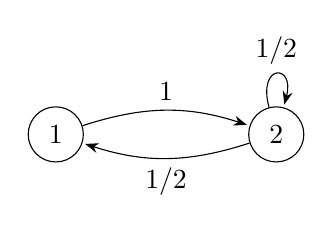
\begin{tikzpicture}[>=Stealth,shorten >=1pt,node distance=2.8cm,on grid,auto,
          every state/.style={minimum size=7mm,inner sep=0pt}]
          \node[state] (s1) {$1$};
          \node[state] (s2) [right=of s1] {$2$};
          \path[->]
            (s1) edge[bend left=18] node[above] {$1$} (s2)
            (s2) edge[loop above] node {$1/2$} (s2)
            (s2) edge[bend left=18] node[below] {$1/2$} (s1);
        \end{tikzpicture}
        \end{center}
        则 $p_{11}^{(2)}$ 等于（\hspace{1.5em}）。

        \fourchoices{$0$}{$1/2$}{$3/4$}{$1$}

  \item 某 Markov 链的状态转移图如下：

        \begin{center}
        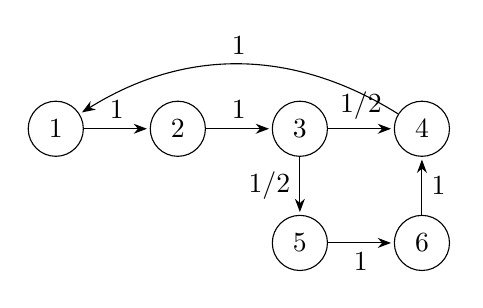
\begin{tikzpicture}[>=Stealth,shorten >=1pt,node distance=1.45cm and 1.55cm,on grid,auto,
          every state/.style={minimum size=7mm,inner sep=0pt}]
          \node[state] (s1) {$1$};
          \node[state] (s2) [right=of s1] {$2$};
          \node[state] (s3) [right=of s2] {$3$};
          \node[state] (s4) [right=of s3] {$4$};
          \node[state] (s5) [below=of s3] {$5$};
          \node[state] (s6) [below=of s4] {$6$};
          \path[->]
            (s1) edge node[above] {$1$} (s2)
            (s2) edge node[above] {$1$} (s3)
            (s3) edge node[above] {$1/2$} (s4)
            (s3) edge node[left] {$1/2$} (s5)
            (s5) edge node[below] {$1$} (s6)
            (s6) edge node[right] {$1$} (s4)
            (s4) edge[bend right=32] node[above] {$1$} (s1);
        \end{tikzpicture}
        \end{center}
        从状态 $1$ 出发，状态 $1$ 的周期为（\hspace{1.5em}）。

        \fourchoices{$1$}{$2$}{$4$}{$6$}

  \item 若有限 Markov 链不可约，且某状态 $i$ 满足 $p_{ii}>0$，则该链（\hspace{1.5em}）。

        \begin{tabularx}{\linewidth}{@{}X X@{}}
          A. 一定周期为 $2$ & B. 一定非周期 \\
          C. 一定有两个平稳分布 & D. 一定非常返
        \end{tabularx}

  \item 对有限不可约非周期 Markov 链，平稳分布为 $\pi$，则下列正确的是（\hspace{1.5em}）。

        \begin{tabularx}{\linewidth}{@{}X X@{}}
          A. $p_{ij}^{(n)}\to0$ & B. $p_{ij}^{(n)}\to\pi_i$ \\
          C. $p_{ij}^{(n)}\to\pi_j$ & D. 极限一定依赖初始状态
        \end{tabularx}
\end{enumerate}

\sectiontitle{三、填空题（每题 2 分，共 10 分）}
\begin{enumerate}
  \item 若 $\mathbb{E}(X\mid Y=y)=g(y)$，则随机变量形式的条件期望为
        $\mathbb{E}(X\mid Y)=$\blank[5cm]。
  \item 某地每天的天气只有“晴”和“雨”。若今天晴，则明天晴的概率为 $0.8$；若今天雨，则明天雨的概率为 $0.6$。假设天气变化构成齐次 Markov 链。已知今天晴，则后天仍为晴天的概率为\blank[3cm]。
\end{enumerate}

\newpage
%============================== 第 3 页 ==============================
\begin{enumerate}[start=3]
  \item 强度为 $\lambda$ 的 Poisson 过程中，第 $k$ 个到达时间 $T_k$ 的期望为\blank[4cm]。
  \item Markov 链的 Chapman--Kolmogorov 方程为
        \[
          p_{ij}^{(m+n)}=\blank[7cm]\text{。}
        \]
  \item 概率向量 $\pi$ 是 Markov 链的平稳分布，当且仅当
        \blank[4cm]，$\displaystyle\sum_j\pi_j=1$。
\end{enumerate}

\sectiontitle{四、计算题（每题 10 分，共 40 分）}
\begin{enumerate}
  \item 设
        \[
          X(t)=A\cos t+B\sin t,\qquad t\in\mathbb{R},
        \]
        其中 $A,B$ 相互独立，且
        \[
          \mathbb{E}A=\mathbb{E}B=0,\qquad \operatorname{Var}(A)=\operatorname{Var}(B)=1\text{。}
        \]
        求：
        \begin{enumerate}[label=(\arabic*),leftmargin=2.2em]
          \item 均值函数 $m_X(t)=\mathbb{E}X(t)$；
          \item 协方差函数 $R_X(s,t)=\operatorname{Cov}(X(s),X(t))$；
          \item 判断该过程是否宽平稳，并说明理由。
        \end{enumerate}

        \workarea{6cm}

  \item 某服务台顾客到达服从强度为 $4$ 人/小时的 Poisson 过程 $N(t)$。
        \begin{enumerate}[label=(\arabic*),leftmargin=2.2em]
          \item 求 $30$ 分钟内恰好到达 $3$ 人的概率；
          \item 求从营业开始第一位顾客到达超过 $15$ 分钟的概率；
          \item 已知 $1$ 小时内恰好到达 $6$ 人，求前 $20$ 分钟内恰好到达 $2$ 人的概率。
        \end{enumerate}

        \workarea{3.8cm}
\end{enumerate}

\newpage
%============================== 第 4 页 ==============================
\begin{enumerate}[start=3]
  \item 某系统有状态空间 $S=\{1,2,3\}$，一步转移矩阵为
        \[
          P=\begin{pmatrix}
            1/2 & 1/2 & 0\\
            1/4 & 1/2 & 1/4\\
            0   & 1/2 & 1/2
          \end{pmatrix}\text{。}
        \]
        \begin{enumerate}[label=(\arabic*),leftmargin=2.2em]
          \item 计算二步转移矩阵 $P^2$；
          \item 若 $X_0=1$，求 $\mathbb{P}(X_2=3)$；
          \item 求初始分布 $\mu^{(0)}=(1/2,1/2,0)$ 经过 $2$ 步后的分布 $\mu^{(2)}$。
        \end{enumerate}

        \workarea{14cm}
\end{enumerate}

\newpage
%============================== 第 5 页 ==============================
\begin{enumerate}[start=4]
  \item 设 Markov 链的状态空间为 $S=\{1,2,3\}$，转移矩阵为
        \[
          P=\begin{pmatrix}
            1/2 & 1/2 & 0\\
            1/4 & 1/2 & 1/4\\
            0   & 1/2 & 1/2
          \end{pmatrix}\text{。}
        \]
        \begin{enumerate}[label=(\arabic*),leftmargin=2.2em]
          \item 判断该链是否不可约、是否非周期；
          \item 求其平稳分布 $\pi$；
          \item 写出 $\displaystyle\lim_{n\to\infty}p_{13}^{(n)}$。
        \end{enumerate}

        \workarea{5.8cm}
\end{enumerate}

\sectiontitle{五、应用题（每题 10 分，共 20 分）}
\begin{enumerate}
  \item 某呼叫中心接到电话服从强度为 $12$ 次/小时的 Poisson 过程。每个电话独立地以概率 $1/4$ 被分配到技术支持组，其余分配到普通客服组。
        \begin{enumerate}[label=(\arabic*),leftmargin=2.2em]
          \item 说明技术支持组接到的电话过程是什么过程，并给出其强度；
          \item 求 $2$ 小时内技术支持组恰好接到 $4$ 个电话的概率；
          \item 求 $2$ 小时内普通客服组接到电话数的期望。
        \end{enumerate}

        \workarea{7.5cm}
\end{enumerate}

\newpage
%============================== 第 6 页 ==============================
\begin{enumerate}[start=2]
  \item 某品牌连锁餐厅在品牌 $A,B$ 之间进行试验。按照时间顺序记录到如下状态序列：
        \[
          B,A,A,A,A,B,B,B,B,A,A,A,A,B,B,B,B,A,A,A\text{。}
        \]
        假设品牌选择可用状态空间 $S=\{A,B\}$ 上的齐次一阶 Markov 链近似描述，并用相邻观测频数的观测频率估计转移概率。
        \begin{enumerate}[label=(\arabic*),leftmargin=2.2em]
          \item 统计 $A\to A$、$A\to B$、$B\to A$、$B\to B$ 四种相邻转移的次数，并据此写出以 $(A,B)$ 为状态顺序的一步转移概率矩阵；
          \item 求该转移矩阵的平稳分布；
          \item 若该经验转移规律长期保持，求从长期看 $A,B$ 的市场份额分别为多少？
        \end{enumerate}

        \workarea{16cm}
\end{enumerate}

\begin{center}
  —— 试卷结束 ——
\end{center}

\end{document}
